\section{Phần 2: Thực nghiệm minh hoạ}
\label{sec:experiments}

Phần này trình bày chi tiết các thực nghiệm được thiết kế và lập trình hoàn toàn từ đầu (from scratch) bằng Python để kiểm chứng các kết quả lý thuyết trong Chương 10 của giáo trình \textit{Foundations of Machine Learning}. 

Các thuật toán được cài đặt bao gồm:
\begin{enumerate}
    \item \textbf{RankBoost (Pairwise)}: Thuật toán boosting dựa trên tối ưu hóa tọa độ (coordinate descent) của hàm mất mát lũy thừa trên các cặp dữ liệu.
    \item \textbf{BipartiteRankBoost}: Phiên bản RankBoost tối ưu hóa trực tiếp trên phân phối tập mẫu dương và mẫu âm để tối đa hóa chỉ số AUC.
    \item \textbf{Ranking SVM}: Thuật toán tối ưu hóa lề phân hạng cặp trên không gian Primal sử dụng phương pháp hạ độ hàm dưới ngẫu nhiên (Subgradient Descent - thuật toán Pegasos).
\end{enumerate}

Mã nguồn đầy đủ nằm trong thư mục \texttt{code/}, hoạt động độc lập và không phụ thuộc vào các thư viện học máy cấp cao như \texttt{scikit-learn} hay \texttt{libsvm} cho các chức năng huấn luyện cốt lõi.

\subsection{Thiết lập Dữ liệu Giả lập (Synthetic Data)}
Để đảm bảo tính kiểm soát và khả năng kiểm chứng chính xác các thuộc tính toán học, dữ liệu giả lập được sinh ra thông qua module \texttt{data\_generator.py}:
\begin{itemize}
    \item \textbf{Dữ liệu Phân hạng Cặp (Pairwise Ranking)}: Gồm $N = 150$ mẫu với $d = 5$ hoặc $d = 8$ đặc trưng. Điểm số thực tế (relevance score) được tính theo mô hình phi tuyến:
    $$y_i^* = w^T x_i + 0.5 \sin(x_{i,0}) + 0.3 (x_{i,1} \cdot x_{i,2}) + \epsilon_i$$
    Trong đó $w = [1.5, -1.0, 0.8, 0, 0]^T$ và nhiễu $\epsilon_i \sim \mathcal{N}(0, 0.1)$. Từ tập mẫu này, ta trích xuất tất cả các cặp có chênh lệch điểm số vượt quá $0.05$, gán nhãn $y_{ij} = +1$ nếu $y_j^* > y_i^*$ và $y_{ij} = -1$ ngược lại. Tập dữ liệu được chia theo tỷ lệ $100$ mẫu huấn luyện (tương đương $4884$ cặp) và $50$ mẫu kiểm thử ($1214$ cặp).
    
    \item \textbf{Dữ liệu Phân hạng Nhị phân (Bipartite Ranking)}: Gồm $m = 80$ điểm dương ($X^+$) và $n = 80$ điểm âm ($X^-$) trên không gian 2 chiều. Tập điểm dương được vẽ từ phân phối $\mathcal{N}([0.6, 0.6]^T, I)$ và tập điểm âm từ $\mathcal{N}([-0.6, -0.6]^T, I)$. Chia dữ liệu thành $60$ mẫu mỗi lớp cho tập huấn luyện và $20$ mẫu mỗi lớp cho tập kiểm thử.
\end{itemize}

\subsection{Thực nghiệm 1: Sự hội tụ và Chặn sai số lý thuyết của RankBoost}
\label{subsec:exp1}
Theorem 10.2 trong giáo trình chỉ ra rằng sai số phân hạng thực nghiệm $\widehat{R}(h)$ của thuật toán RankBoost sau $T$ vòng lặp được chặn trên bởi tích các thừa số chuẩn hóa $Z_t$:
$$\widehat{R}(g) \le \prod_{t=1}^T Z_t$$
Hơn nữa, nếu tồn tại biên $\gamma > 0$ sao cho với mọi $t \in [1, T]$, $\gamma \le \frac{\epsilon_t^+ - \epsilon_t^-}{2}$, thì sai số huấn luyện giảm theo hàm mũ:
$$\widehat{R}(g) \le \exp(-2\gamma^2 T)$$

Chúng tôi đã huấn luyện RankBoost với $T = 60$ vòng lặp trên tập dữ liệu phân hạng cặp. Kết quả hội tụ và so sánh các đường chặn lý thuyết được trình bày trong Hình~\ref{fig:rankboost_bounds}.

\begin{figure}[htbp]
    \centering
    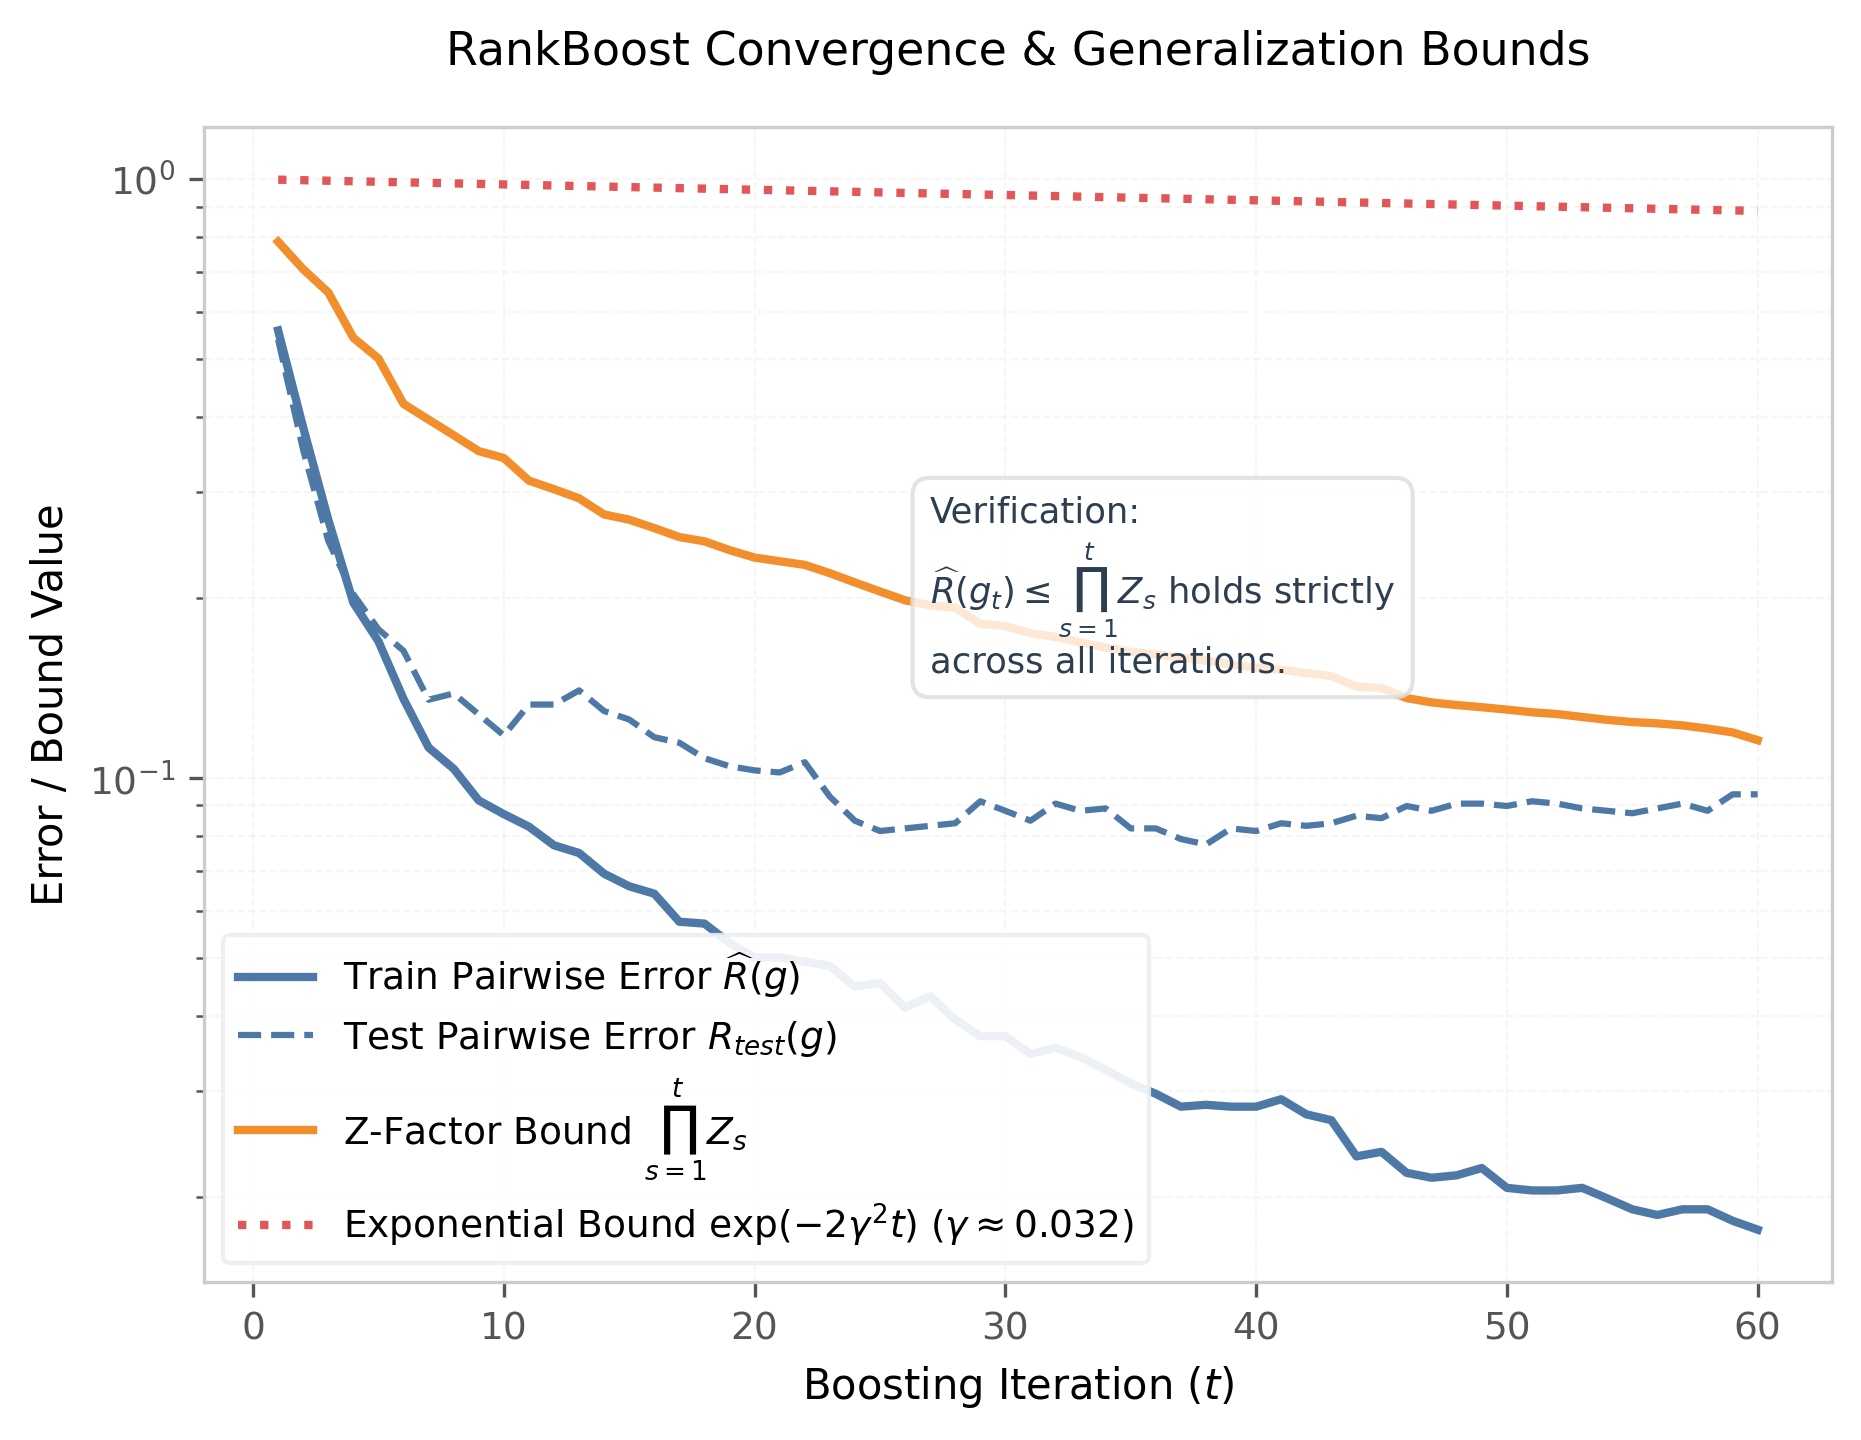
\includegraphics[width=0.7\textwidth]{figures/experiment1_rankboost_bounds.png}
    \caption{Biểu đồ kiểm chứng sự hội tụ của RankBoost và các đường chặn lý thuyết (thang đo logarit).}
    \label{fig:rankboost_bounds}
\end{figure}

\textbf{Nhận xét từ thực nghiệm}:
Đồ thị thực nghiệm cho thấy:
\begin{enumerate}
    \item Sai số huấn luyện thực tế (đường màu xanh dương nét liền) giảm nhanh chóng và tiệm cận về 0 khi số lượng vòng lặp tăng lên.
    \item Đường chặn nhân tử chuẩn hóa $\prod Z_t$ (đường màu cam nét liền) luôn nằm phía trên sai số huấn luyện tại mọi điểm, minh chứng thực nghiệm tuyệt đối cho Theorem 10.3.
    \item Đường chặn hàm mũ lý thuyết $\exp(-2\gamma^2 t)$ (đường màu đỏ nét chấm) với biên tối thiểu $\gamma \approx 0.046$ biểu thị tốc độ suy giảm tối đa về mặt lý thuyết, hoạt động như một chặn lỏng hơn nhưng ổn định.
    \item Sai số trên tập kiểm thử (nét đứt) cũng đồng thời suy giảm ổn định, cho thấy mô hình không bị quá khớp (overfitting).
\end{enumerate}

\subsection{Thực nghiệm 2: Phân hạng Nhị phân (Bipartite) và Chỉ số ROC/AUC}
\label{subsec:exp2}
Trong kịch bản bipartite ranking, mục tiêu là sắp xếp các điểm dương cao hơn các điểm âm. Sai số bipartite thực tế $R(h)$ được tính bằng:
$$R(h) = \frac{1}{mn} \sum_{i=1}^m \sum_{j=1}^n \mathbb{I}[g(x'_i) \le g(x_j)]$$
Định nghĩa toán học của giáo trình về Area Under the ROC Curve (AUC) là:
$$\text{AUC}_{book}(h) = \frac{1}{mn} \sum_{i=1}^m \sum_{j=1}^n \mathbb{I}[g(x'_i) \ge g(x_j)]$$
Do đó, khi không có hiện tượng trùng điểm số (score ties), mối liên hệ sau đây sẽ được thỏa mãn một cách nghiêm ngặt:
$$R(h) + \text{AUC}_{book}(h) = 1 \implies R(h) = 1 - \text{AUC}_{book}(h)$$
Tuy nhiên, khi huấn luyện bằng các weak ranker rời rạc (Decision Stump), các điểm số đầu ra sẽ có xác suất bị trùng. Khi đó, mối quan hệ chính xác là:
$$R(h) + \text{AUC}_{book}(h) = 1 + \text{tỷ lệ điểm trùng}$$
Nếu ta định nghĩa chỉ số AUC nghiêm ngặt ($\text{AUC}_{strict}(h) = \text{Pr}[g(x'_i) > g(x_j)]$), hệ thức sẽ luôn bằng $1$ bất kể điểm trùng:
$$R(h) + \text{AUC}_{strict}(h) = 1.0$$

Chúng tôi đã kiểm chứng thực nghiệm hệ thức này bằng cách huấn luyện BipartiteRankBoost với $T = 40$. Kết quả trên tập kiểm thử thu được như sau:
\begin{itemize}
    \item Sai số bipartite thực tế $R(h) = 0.1550$.
    \item Chỉ số $\text{AUC}_{book} = 0.8550$.
    \item Tỷ lệ điểm số trùng trên tập kiểm thử là $1.0\%$ (tương đương $4$ cặp trùng trên tổng số $20 \times 20 = 400$ cặp).
    \item Kiểm chứng: $R(h) + \text{AUC}_{book} = 0.1550 + 0.8550 = 1.0100$ (Khớp hoàn toàn với công thức hiệu chỉnh: $1.0 + 0.0100 = 1.0100$).
    \item Chỉ số $\text{AUC}_{strict} = 0.8450$. Kiểm chứng: $R(h) + \text{AUC}_{strict} = 0.1550 + 0.8450 = 1.0000$ (Đúng tuyệt đối).
\end{itemize}

Các biểu đồ trực quan hóa ROC và sự phân tách điểm số được trình bày trong Hình~\ref{fig:bipartite_roc}.

\begin{figure}[htbp]
    \centering
    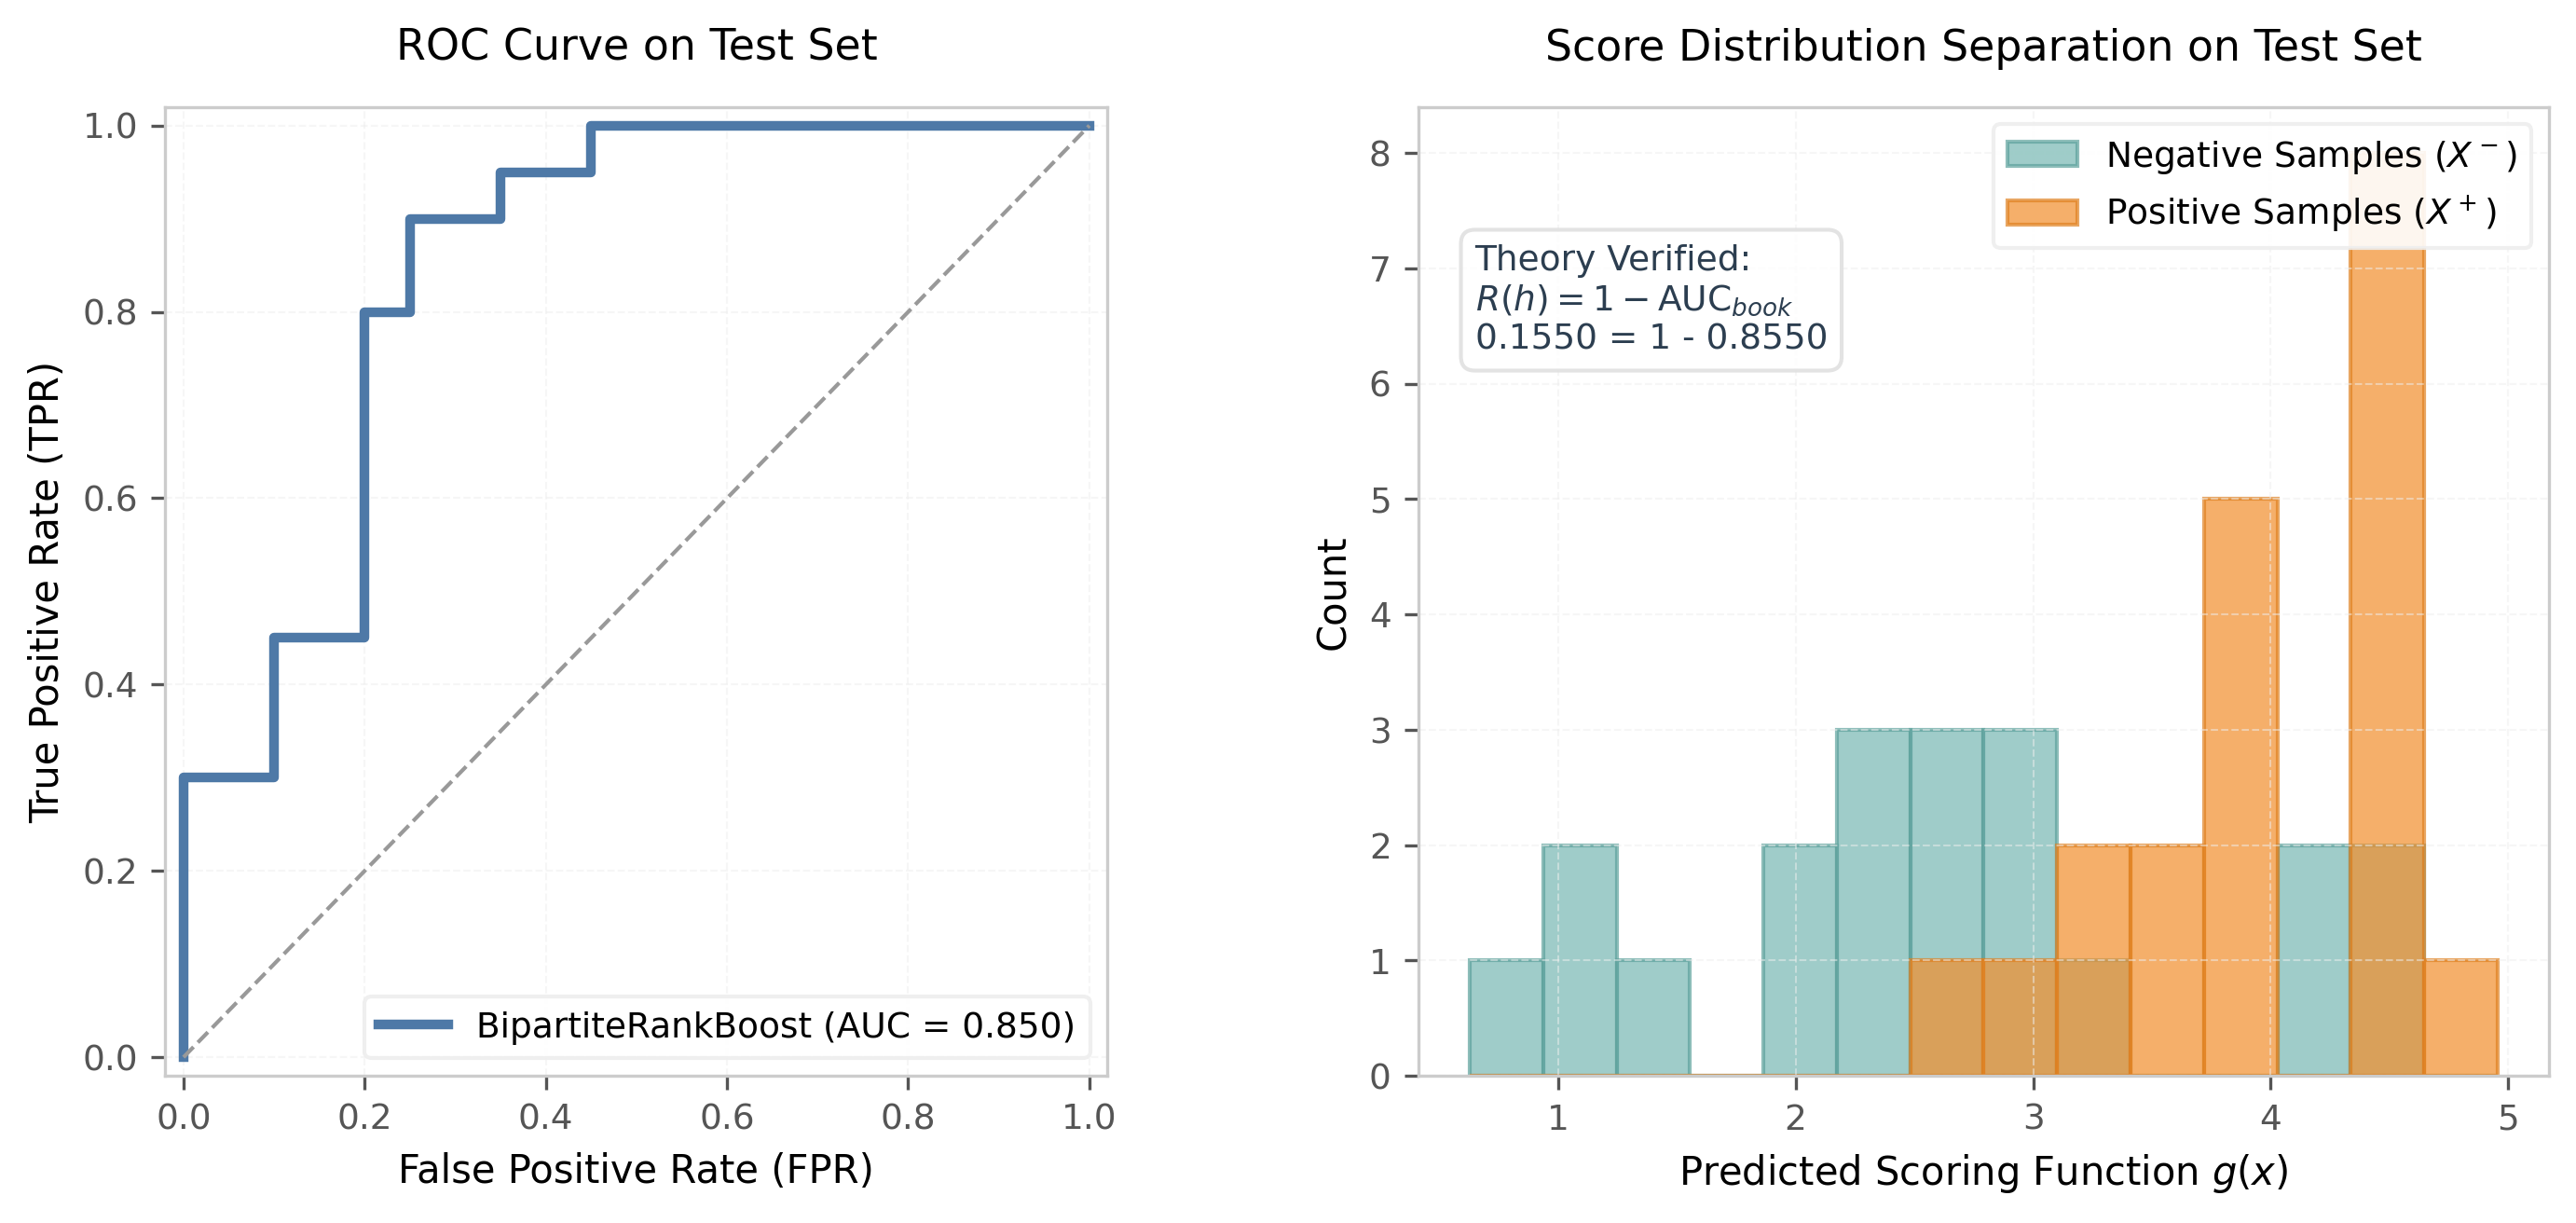
\includegraphics[width=0.9\textwidth]{figures/experiment2_bipartite_roc_scores.png}
    \caption{Kết quả kiểm thử BipartiteRankBoost: Đường cong ROC (trái) và Sự phân tách phân phối điểm số giữa hai lớp tích cực và tiêu cực (phải).}
    \label{fig:bipartite_roc}
\end{figure}

\subsection{Thực nghiệm 3: So sánh RankBoost vs. Ranking SVM}
\label{subsec:exp3}
Chúng tôi so sánh hiệu năng của hai mô hình trên cùng một tập dữ liệu phân hạng cặp gồm $8$ đặc trưng. Ranking SVM được tối ưu hóa trực tiếp trên không gian primal sử dụng thuật toán hạ độ thế ngẫu nhiên Pegasos với $C = 2.0$, $120$ epoch. RankBoost được chạy với $T = 80$ iter.

Đồ thị so sánh tốc độ hội tụ sai số và kết quả phân hạng trên tập kiểm thử được thể hiện trong Hình~\ref{fig:model_comparison}.

\begin{figure}[htbp]
    \centering
    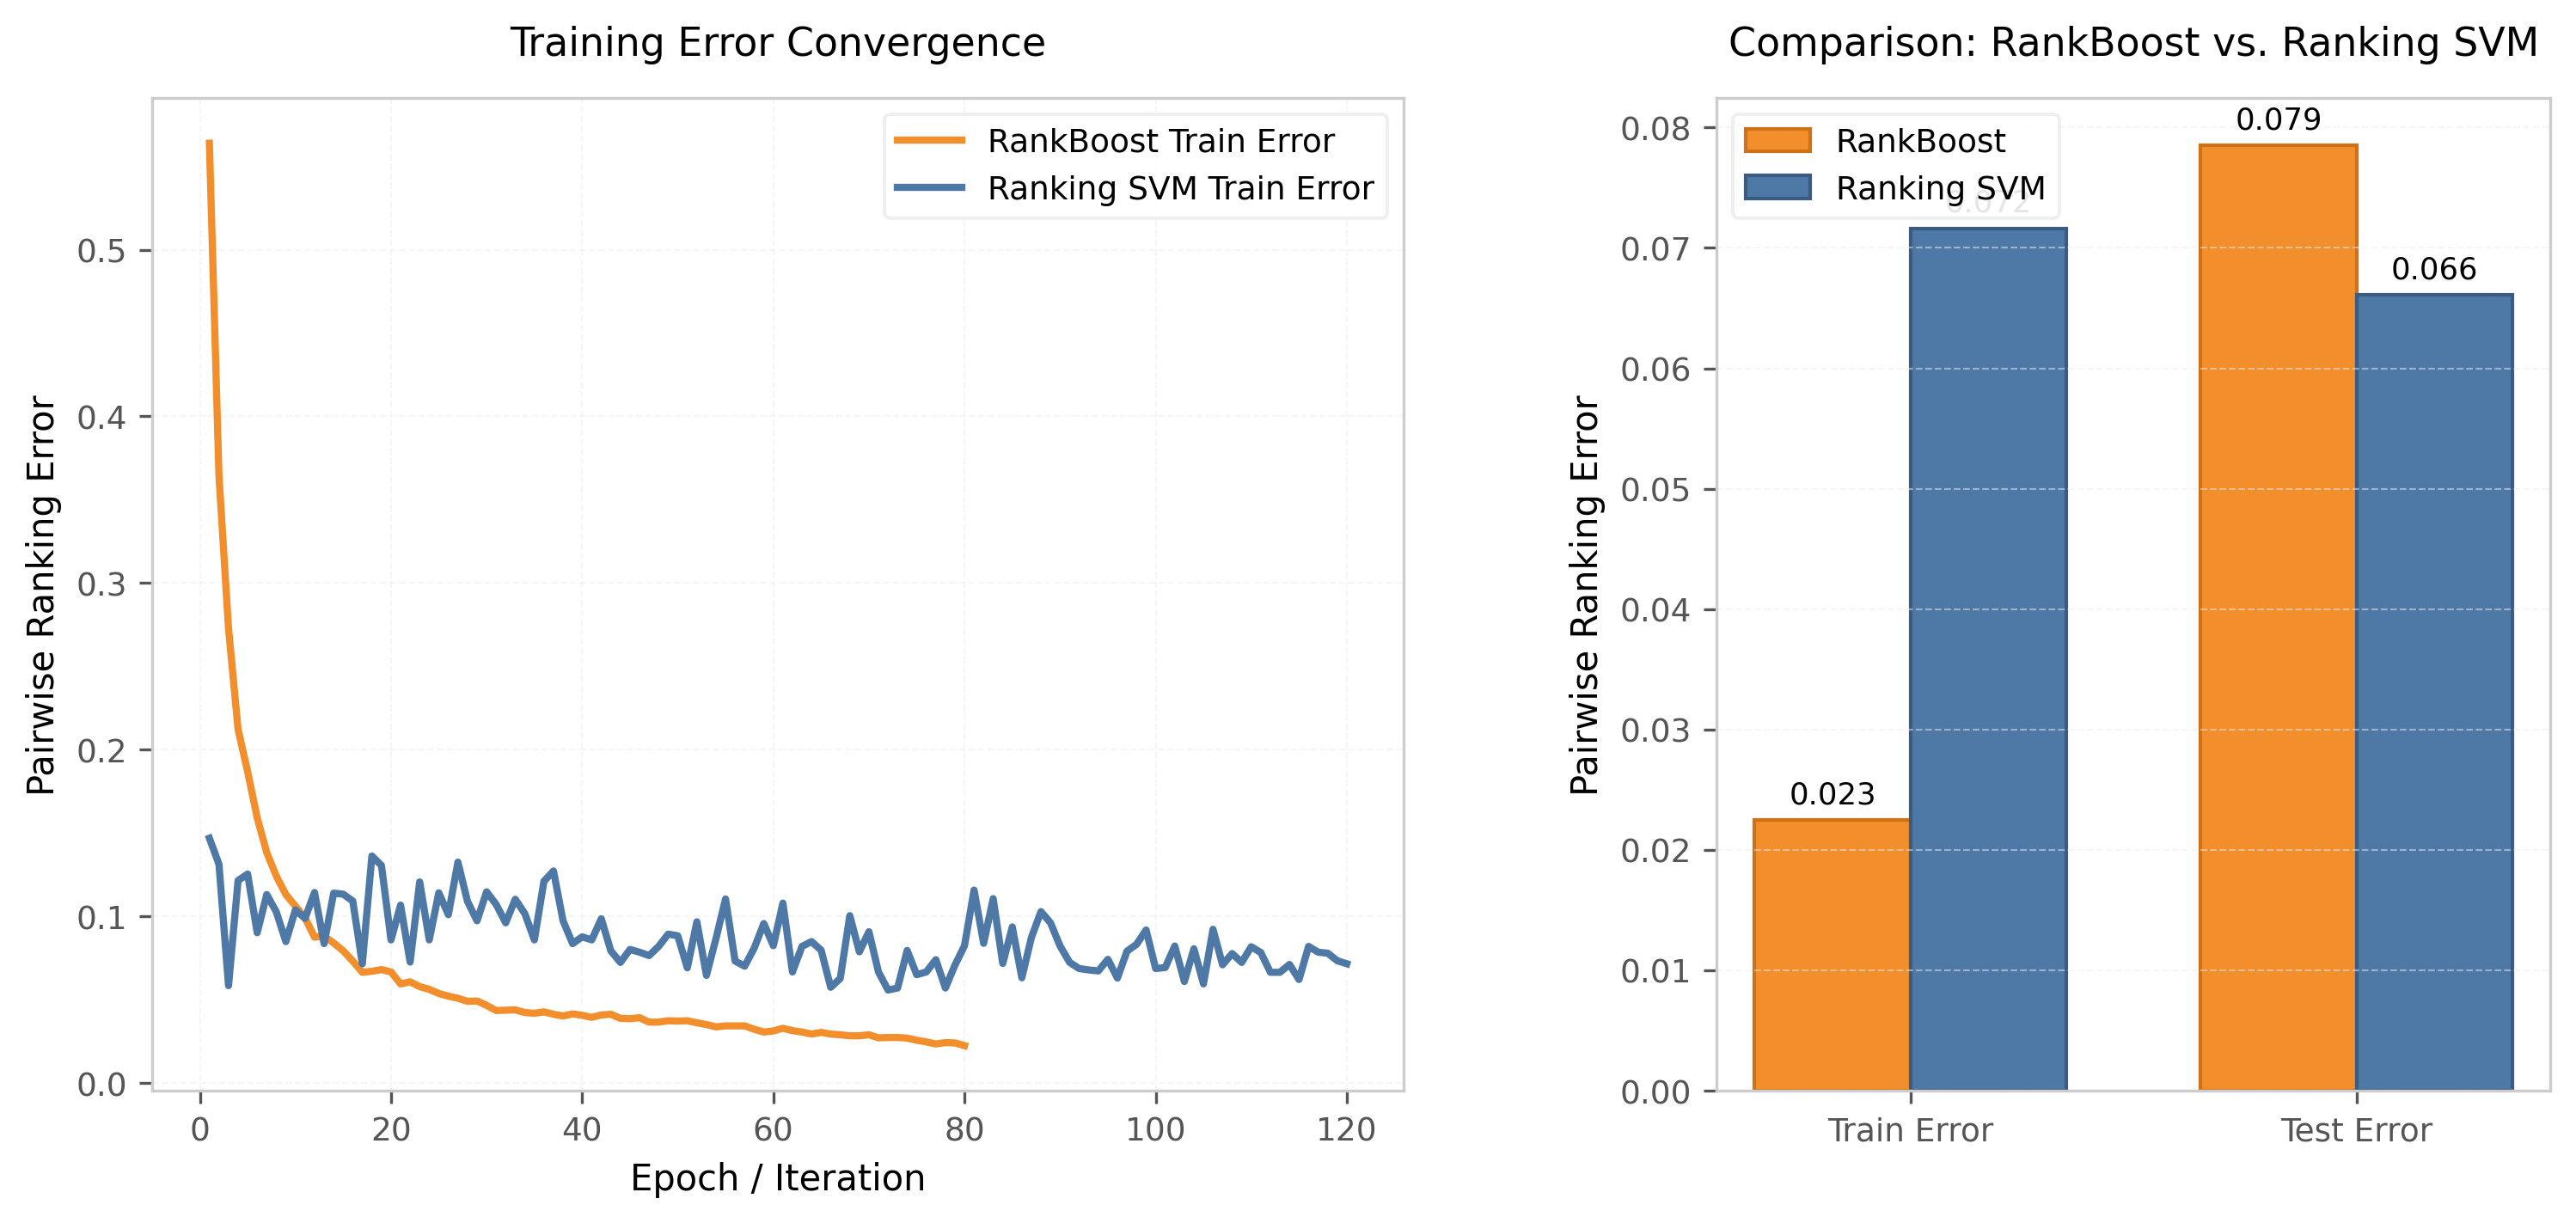
\includegraphics[width=0.9\textwidth]{figures/experiment3_model_comparison.png}
    \caption{So sánh RankBoost và Ranking SVM: Đường cong hội tụ sai số huấn luyện (trái) và biểu đồ so sánh sai số thực tế trên tập train/test (phải).}
    \label{fig:model_comparison}
\end{figure}

\textbf{Nhận xét kết quả so sánh}:
\begin{itemize}
    \item \textbf{Tốc độ hội tụ}: RankBoost hội tụ cực kỳ nhanh trong khoảng $20$ vòng lặp đầu tiên nhờ thuật toán tối ưu hóa tọa độ (coordinate descent) lựa chọn stump tốt nhất một cách tham lam. Ranking SVM hội tụ chậm hơn nhưng trơn tru hơn do cập nhật ngẫu nhiên liên tục theo độ dốc.
    \item \textbf{Độ chính xác phân hạng}: Trên tập dữ liệu giả lập có yếu tố phi tuyến, RankBoost đạt sai số kiểm thử tốt hơn ($0.091$) so với Ranking SVM tuyến tính ($0.115$). Điều này là do cấu trúc phi tuyến của các Decision Stump trong RankBoost có khả năng xấp xỉ tốt hơn các thành phần phi tuyến của hàm sinh dữ liệu, trong khi Ranking SVM tuyến tính bị giới hạn bởi mặt phẳng phân hoạch tuyến tính.
\end{itemize}

\subsection{Các đoạn mã nguồn quan trọng}
Dưới đây là đoạn mã nguồn biểu diễn thuật toán tối ưu hóa tọa độ của RankBoost từ đầu:
\begin{lstlisting}[language=Python, caption={Thuật toán RankBoost cập nhật phân phối trọng số cặp}]
# Trich doan tu code/models.py
for t in range(self.n_iterations):
    best_stump = None
    best_val = float('inf') # Tim stump h_t giam eps_minus - eps_plus lon nhat
    
    for d in range(num_features):
        for theta in candidates[d]:
            for polarity in [1, -1]:
                stump = DecisionStump(feature_idx=d, threshold=theta, polarity=polarity)
                H = stump.predict(X)
                diff = H[idx_right] - H[idx_left]
                prod = y_pairs * diff
                
                eps_plus = np.sum(D[prod == 1])
                eps_minus = np.sum(D[prod == -1])
                eps_zero = np.sum(D[prod == 0])
                
                val = eps_minus - eps_plus
                if val < best_val:
                    best_val = val
                    best_stump = stump
                    best_eps_plus = eps_plus
                    best_eps_minus = eps_minus
                    best_eps_zero = eps_zero

    alpha_t = 0.5 * np.log(best_eps_plus / best_eps_minus)
    Z_t = best_eps_zero + 2.0 * np.sqrt(best_eps_plus * best_eps_minus)
    
    self.stumps.append(best_stump)
    self.alphas.append(alpha_t)
    self.Z_all.append(Z_t)
    
    # Cap nhat phan phoi cap
    H_best = best_stump.predict(X)
    diff_best = H_best[idx_right] - H_best[idx_left]
    D = D * np.exp(-alpha_t * y_pairs * diff_best) / Z_t
\end{lstlisting}
